\documentclass[10pt,aspectratio=169]{beamer}

% ---- Minimal academic theme ----
\usetheme{default}
\usefonttheme{professionalfonts}
\setbeamertemplate{navigation symbols}{}

% Uncomment for presenter mode:
% \usepackage{pgfpages}
% \setbeameroption{show notes on second screen=right}

\usepackage{booktabs}
\usepackage{amsmath}
\usepackage{xcolor}
\usepackage{tikz}
\usetikzlibrary{arrows.meta, positioning}
\usepackage{graphicx}
\usepackage{colortbl}
\usepackage{array}
\usepackage[round,authoryear]{natbib}

% ---- Color palette ----
\definecolor{ink}{RGB}{20,24,31}
\definecolor{muted}{RGB}{100,110,125}
\definecolor{rulegray}{RGB}{200,206,215}
\definecolor{accent}{RGB}{12,64,120}
\definecolor{wingreen}{RGB}{210,245,210}
\definecolor{loserose}{RGB}{255,220,220}
\definecolor{midgray}{RGB}{246,247,249}
\definecolor{lightblue}{RGB}{220,235,255}
% Aliases for content slides
\colorlet{accentblue}{accent}
\definecolor{accentred}{RGB}{160,35,35}

% ---- Beamer colors ----
\setbeamercolor{normal text}{fg=ink,bg=white}
\setbeamercolor{structure}{fg=accent}
\setbeamercolor{frametitle}{fg=ink,bg=white}
\setbeamercolor{title}{fg=ink}
\setbeamercolor{alerted text}{fg=accentred}

% ---- Beamer fonts ----
\setbeamerfont{title}{size=\LARGE,series=\bfseries}
\setbeamerfont{frametitle}{size=\large,series=\bfseries}
\setbeamerfont{footline}{size=\scriptsize}

% ---- Frametitle: bold heading + thin rule ----
\setbeamertemplate{frametitle}{%
  \vspace{0.45em}%
  \textbf{\insertframetitle}\par
  \vspace{0.20em}%
  {\color{rulegray}\rule{\linewidth}{0.35pt}}%
  \vspace{0.10em}%
}

% ---- Footer: author | title on left, slide number on right ----
\setbeamertemplate{footline}{%
  \leavevmode%
  \hbox{%
    \begin{beamercolorbox}[wd=.72\paperwidth,ht=2.25ex,dp=1ex,leftskip=0.55cm]{normal text}%
      \textcolor{muted}{Zeynep Bozoklu \textbar\ Functional Forecasting of Turkish Electricity Load Curves}%
    \end{beamercolorbox}%
    \begin{beamercolorbox}[wd=.28\paperwidth,ht=2.25ex,dp=1ex,rightskip=0.55cm plus1fil]{normal text}%
      \hfill\textcolor{muted}{\insertframenumber\,/\,\inserttotalframenumber}%
    \end{beamercolorbox}%
  }%
}

\setlength{\tabcolsep}{5pt}
\renewcommand{\arraystretch}{1.15}

\title{Functional Forecasting of Turkish Electricity Load Curves}
\subtitle{MRes Thesis Proposal}
\author{Zeynep Bozoklu}
\date{June 2026}

\begin{document}

% ============================================================
% SLIDE 1: TITLE
% ============================================================
\begin{frame}[plain]
  \vspace{0.9cm}
  {\usebeamerfont{title}\usebeamercolor[fg]{title}\inserttitle\par}
  \vspace{0.25em}
  {\small\textcolor{muted}{\insertsubtitle}\par}
  \vspace{0.8em}
  \small
  \begin{tabular}{@{}p{0.20\linewidth}p{0.70\linewidth}@{}}
    \toprule
    Object     & Daily load curve $Y_d(h)$, $h=0,\ldots,23$ (MWh/hour) \\
    Benchmark  & Official day-ahead forecast published by TEİAŞ / EPIAS \\
    Evaluation & Rolling-origin, 2023--2025, 1,096 test days, 26,304 hourly errors \\
    Main test  & Diebold--Mariano (pooled and hour-by-hour) \\
    \bottomrule
  \end{tabular}
  \vfill
  {\small\textbf{Zeynep Bozoklu}\quad\textcolor{muted}{MRes Thesis Proposal \textbar\ June 2026}}
  \note{Introduce the thesis: applying Functional Data Analysis to forecast Turkey's daily electricity load curve. The core preliminary result: the FPCA-VAR model beats the official TEİAŞ benchmark by 19\% MAE with DM p-value near $10^{-163}$, and 46\% after a residual correction. 18 slides, roughly 20 minutes.}
\end{frame}

% ============================================================
% SLIDE 2: THE FORECASTING OBJECT
% ============================================================
\begin{frame}{The Forecasting Object: A Daily Load Curve}
  \begin{columns}
    \begin{column}{0.62\textwidth}
      \includegraphics[width=\linewidth]{../output/figs/fda_mean_actual_forecast_all.png}
    \end{column}
    \begin{column}{0.35\textwidth}
      \Large $Y_d(h),\quad h = 0,\ldots,23$
      \vspace{0.7em}

      \normalsize
      \begin{itemize}
        \item A single \textbf{curve}, not 24 scalars
        \item Dual-peak shape is structurally stable across all days
        \item Solid = actual;\quad dashed = official forecast
        \item \textbf{Goal:} forecast tomorrow's full 24-hour profile
      \end{itemize}

      \vspace{0.7em}
      \small The official forecast (dashed) lies \emph{systematically below}
      the actual --- persistent underprediction at every hour.
    \end{column}
  \end{columns}
  \note{The dual-peak shape is an imprint of human behavior: low overnight, steep morning ramp, industrial plateau, residential evening surge, then decline. The key observation motivating FDA: these 24 numbers are not 24 independent measurements --- they are one coherent trajectory. Treating them as 24 separate forecasting problems throws away all shape information. Note the persistent underprediction of the official (dashed): quantified on slide 4.}
\end{frame}

% ============================================================
% SLIDE 3: THE ECONOMIC STORY OF THE CURVE
% ============================================================
\begin{frame}{The Load Curve Is an Economic Story}
  \begin{columns}
    \begin{column}{0.62\textwidth}
      \small
      \renewcommand{\arraystretch}{1.25}
      \begin{tabular}{p{0.22\linewidth}p{0.12\linewidth}p{0.34\linewidth}p{0.20\linewidth}}
        \toprule
        Segment & Hours & Economic driver & vs.\ official \\
        \midrule
        \rowcolor{midgray}
        Overnight trough
          & 0--5
          & Factories + infra; stable, weekly-seasonal
          & \textcolor{accentblue}{Wins 40--60\%} \\
        \rowcolor{loserose}
        Morning ramp
          & 6--8
          & Demand doubles; ramp \emph{timing} temperature-driven
          & \textcolor{accentred}{Loses (up to 24\%)} \\
        \rowcolor{midgray}
        Midday plateau
          & 9--16
          & Industrial \& commercial peak; weekday-driven
          & \textcolor{accentblue}{Wins 20--35\%} \\
        \rowcolor{loserose}
        Evening surge
          & 17--19
          & Residential peak; AC/heating at max; largest official bias
          & \textcolor{accentred}{Mixed} \\
        \rowcolor{midgray}
        Night wind-down
          & 20--23
          & Smooth decline toward trough
          & \textcolor{accentblue}{Wins 17--20\%} \\
        \bottomrule
      \end{tabular}
    \end{column}
    \begin{column}{0.35\textwidth}
      \small
      \textbf{Why functional analysis fits:}\\[0.4em]
      These 24 observations are one coherent trajectory shaped by
      overlapping behavioral rhythms.

      \vspace{0.4em}
      The morning ramp, midday plateau, and evening peak are
      \emph{features of the whole curve} --- not of individual hours.
      FDA works with these shape features directly via eigenfunctions
      and derivative summaries.

      \vspace{0.5em}
      \textcolor{accentred}{\textbf{Red rows:}} transition segments
      where demand changes fastest and forecasting is hardest.
    \end{column}
  \end{columns}
  \note{This slide builds the intuition for the FDA framework and previews the hour-by-hour results. The morning ramp (6--8) is the most consequential segment: demand doubles within two hours. The ramp timing depends critically on temperature --- the official likely uses weather inputs here, which is why it has an advantage at those hours. The functional approach captures ramp steepness via B-spline derivatives. The evening surge (17--19) is where the official underpredicts most severely: average bias 614--658 MWh.}
\end{frame}

% ============================================================
% SLIDE 4: WHY ACCURACY MATTERS
% ============================================================
\begin{frame}{Why Accuracy Matters}
  \begin{columns}
    \begin{column}{0.44\textwidth}
      \textbf{Key users (post-2013 liberalisation):}
      \vspace{0.3em}
      \begin{itemize}
        \item \textbf{TEİAŞ} (transmission system operator)\\
              {\small unit commitment, reserve scheduling}
        \item \textbf{Generators}\\
              {\small day-ahead market bids on EPIAS}
        \item \textbf{Large consumers}\\
              {\small real-time imbalance penalties}
      \end{itemize}

      \vspace{0.5em}
      \textbf{Why does the official underpredict?}\\[0.3em]
      \small Most likely: \textbf{model staleness.} Official systems require
      regulatory approval to update; a model calibrated on older demand
      patterns underpredicts during structural demand growth.\\[0.2em]
      Our rolling-origin re-trains before every step ---
      2024 bias: \textbf{34 MWh} vs.\ official \textbf{585 MWh}.
    \end{column}
    \begin{column}{0.53\textwidth}
      \begin{center}
        \small\textbf{Systematic underprediction: official TEİAŞ forecast}\\[0.4em]
        \begin{tabular}{lrr}
          \toprule
          Year & Official bias & Our bias \\
               & (MWh/hour) & (MWh/hour) \\
          \midrule
          2023 & $+344$ & $+176$ \\
          2024 & $+585$ & $+34$  \\
          2025 & $+472$ & $+98$  \\
          \midrule
          \textbf{Average} & $\mathbf{+467}$ & $\mathbf{+103}$ \\
          \bottomrule
        \end{tabular}\\[0.4em]
        \small Positive bias = forecast $<$ actual (underprediction).
      \end{center}
    \end{column}
  \end{columns}
  \note{The 2024 spike (+585 MWh) coincides with an exceptionally hot Turkish summer driving unusually high AC demand. Our rolling-origin design continuously incorporates the most recent data, so our 2024 bias is only 34 MWh. The most defensible explanation for the persistent official underprediction is model staleness during a period of structural demand growth. Do not speculate beyond what the data shows.}
\end{frame}

% ============================================================
% SLIDE 5: RESEARCH QUESTIONS
% ============================================================
\begin{frame}{Research Questions}
  \begin{enumerate}
    \item \textbf{Representation.} Can B-spline smoothing and FPCA represent
          Turkey's daily electricity load curves with negligible information loss?
          How many functional principal components suffice?

    \vspace{0.5em}
    \item \textbf{Forecasting accuracy.} Does a functional VAR model augmented
          with holiday and derivative features statistically outperform the
          official TEİAŞ day-ahead forecast?\\
          {\small Evaluated by Diebold-Mariano over 1,096 hold-out days, 2023--2025.}

    \vspace{0.5em}
    \item \textbf{Nonlinearity.} Within the FPCA framework, does replacing OLS with
          a nonlinear learner (Random Forest) improve forecast accuracy?
          And does bypassing the functional representation altogether ---
          forecasting each hour directly --- offer further gains?\\
          {\small Preliminary evidence from a one-year subsample raises this as an open question for the thesis.}
  \end{enumerate}
  \note{Three questions. Q1: answered --- 97.3\% variance with K=2. Q2: answered --- +19.2\% over 2023--2025, DM $p \approx 10^{-163}$. Q3: partially answered. Within the FPCA structure, FPCA-RF (MAE 1217) does not improve on FPCA-OLS (MAE 980) and merely ties the official --- OLS regularisation wins. But Direct RF, bypassing FPCA entirely, achieves MAE 718 vs.\ official 1052 on the 2025 subsample (+31.8\%). This is a suggestive preliminary result that motivates extending the nonlinear comparison to the full three-year evaluation window.}
\end{frame}

% ============================================================
% SLIDE 6: LITERATURE
% ============================================================
\begin{frame}{Literature Review}
  \vspace{0.4em}
  \begin{center}
    {\large\textcolor{muted}{\textit{Systematic review in progress.}}}
  \end{center}

  \vspace{0.6em}
  \textbf{Established so far:}
  \begin{itemize}
    \item No FDA-based study of Turkish electricity demand exists in the literature.
  \end{itemize}

  \vspace{0.7em}
  \textbf{Areas to be covered in the full review:}
  \vspace{0.2em}
  \begin{itemize}
    \item Functional Data Analysis foundations and forecasting methods
          (Ramsay \& Silverman 2005; Kokoszka \& Reimherr 2017; Hyndman \& Ullah 2007)
    \item FDA applied to electricity load curves and energy demand
    \item Short-term load forecasting: classical (ARIMA) and machine learning approaches
    \item Turkish electricity market structure post-2013 liberalisation
    \item Residual correction and error correction in forecast combination
          (Xie \& Hong 2016)
  \end{itemize}
  \note{The systematic literature review is the primary remaining task. The one fact already established is that no FDA study of Turkish electricity demand exists --- this defines the gap. The full review will situate the methodology within the FDA forecasting literature and the broader electricity forecasting literature, and will assess what is known about nonlinear load forecasting methods. Be transparent with the committee that this work is ongoing.}
\end{frame}

% ============================================================
% SLIDE 7: THE FDA PIPELINE
% ============================================================
\begin{frame}{From 24 Numbers to a Curve: The FDA Pipeline}
  \vspace{-0.2em}
  \begin{center}
  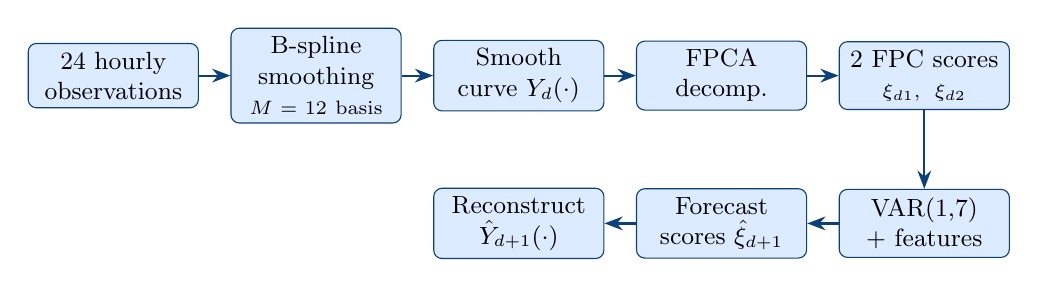
\begin{tikzpicture}[
    node distance=0.45cm and 0.40cm,
    box/.style={rectangle, rounded corners=3pt, draw=accentblue, fill=lightblue,
                text width=1.95cm, align=center, font=\small,
                minimum height=0.78cm, inner sep=3pt},
    arr/.style={-Stealth, thick, accentblue}
  ]
    \node[box] (raw)    {24 hourly\\observations};
    \node[box, right=of raw]    (spline) {B-spline\\smoothing\\{\scriptsize $M=12$ basis}};
    \node[box, right=of spline] (curve)  {Smooth\\curve $Y_d(\cdot)$};
    \node[box, right=of curve]  (fpca)   {FPCA\\decomp.};
    \node[box, right=of fpca]   (scores) {2 FPC scores\\{\scriptsize $\xi_{d1},\;\xi_{d2}$}};

    \node[box, below=1.0cm of scores] (var)   {VAR(1,7)\\$+$ features};
    \node[box, left=of var]           (hatsc) {Forecast\\scores $\hat\xi_{d+1}$};
    \node[box, left=of hatsc]         (recon) {Reconstruct\\$\hat{Y}_{d+1}(\cdot)$};

    \draw[arr] (raw)    -- (spline);
    \draw[arr] (spline) -- (curve);
    \draw[arr] (curve)  -- (fpca);
    \draw[arr] (fpca)   -- (scores);
    \draw[arr] (scores) -- (var);
    \draw[arr] (var)    -- (hatsc);
    \draw[arr] (hatsc)  -- (recon);
  \end{tikzpicture}
  \end{center}
  \vspace{0.5em}
  \begin{columns}
    \begin{column}{0.33\textwidth}
      \centering\small\textbf{B-splines ($M=12$)}\\
      preserves shape; enables differentiation of the curve
    \end{column}
    \begin{column}{0.33\textwidth}
      \centering\small\textbf{FPCA ($K=2$)}\\
      2 scores carry 97.3\% of all curve variation
    \end{column}
    \begin{column}{0.33\textwidth}
      \centering\small\textbf{VAR(1,7) by OLS}\\
      daily + weekly score dynamics
    \end{column}
  \end{columns}
  \note{Walk through the boxes left to right, then down and back. Core compression: instead of 24 separate forecasting models, reduce to 2 scores, forecast those, reconstruct the full curve. B-spline smoothing enables differentiation --- the derivative captures ramp speed at hours 6--8 and 17--19, which becomes a feature in the VAR. Both FPCA and VAR are re-estimated from scratch at every rolling-origin step using only past data.}
\end{frame}

% ============================================================
% SLIDE 8: DATA
% ============================================================
\begin{frame}{Data}
  \begin{columns}
    \begin{column}{0.55\textwidth}
      \begin{center}
      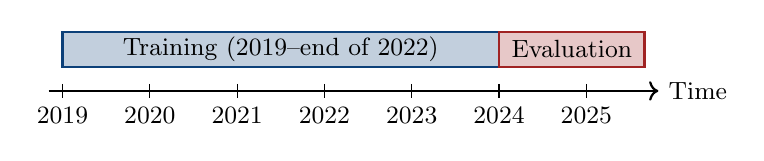
\begin{tikzpicture}[scale=0.88]
        \draw[->, thick] (-0.2,0) -- (8.6,0) node[right,font=\small] {Time};
        \draw[fill=accentblue!25, draw=accentblue, thick]
              (0,0.35) rectangle (6.3,0.85);
        \node[font=\small] at (3.15,0.60) {Training (2019--end of 2022)};
        \draw[fill=accentred!25, draw=accentred, thick]
              (6.3,0.35) rectangle (8.4,0.85);
        \node[font=\small] at (7.35,0.60) {Evaluation};
        \foreach \x/\y in {0/2019, 1.26/2020, 2.52/2021,
                           3.78/2022, 5.04/2023, 6.3/2024, 7.56/2025} {
          \draw (\x,0.1) -- (\x,-0.1) node[below,font=\small] {\y};
        }
      \end{tikzpicture}
      \end{center}
      \vspace{0.4em}
      \small Rolling-origin: model re-estimated before every forecast day
      using only past data. Expanding window --- appropriate because
      eigenfunction shapes are stable across sub-periods.
    \end{column}
    \begin{column}{0.42\textwidth}
      \small
      \begin{tabular}{ll}
        \toprule
        \textbf{Series} & \textbf{Source} \\
        \midrule
        Hourly load (MWh) & EPIAS \\
        Official forecast  & TEİAŞ / EPIAS \\
        Holiday calendar   & Official gazette \\
        \bottomrule
      \end{tabular}
      \vspace{0.7em}

      \begin{tabular}{ll}
        \toprule
        \textbf{Item} & \textbf{Value} \\
        \midrule
        Frequency          & Hourly \\
        Coverage           & 2019--2025 \\
        Training curves    & $\approx$1,460 days \\
        Evaluation curves  & 1,096 days \\
        Hourly errors eval & 26,304 \\
        \bottomrule
      \end{tabular}
    \end{column}
  \end{columns}
  \note{Data from EPIAS via public API. Having both actual load and the official TEİAŞ day-ahead forecast is essential: it provides a directly comparable operational benchmark on the same target days. Expanding window is used because FPCA eigenfunctions are empirically stable across sub-periods (pairwise inner products all exceed 0.99), so all historical data is informative.}
\end{frame}

% ============================================================
% SLIDE 9: FPCA
% ============================================================
\begin{frame}{FPCA: Two Scores Capture the Curve}
  \begin{columns}
    \begin{column}{0.60\textwidth}
      \includegraphics[width=\linewidth]{../output/figs/eigenfunction_shape_comparison.png}
    \end{column}
    \begin{column}{0.37\textwidth}
      \small
      \begin{tabular}{rrr}
        \toprule
        FPC & Variance & Cumulative \\
        \midrule
        1 & 93.4\% & 93.4\% \\
        2 &  3.9\% & 97.3\% \\
        3 &  1.1\% & 98.4\% \\
        4 &  1.0\% & 99.4\% \\
        \bottomrule
      \end{tabular}

      \vspace{0.5em}
      \textbf{FPC 1 --- Level}\\
      {\small Nearly flat $\Rightarrow$ shifts the whole curve up or down uniformly.}

      \vspace{0.4em}
      \textbf{FPC 2 --- Shape contrast}\\
      {\small Positive overnight \& evening, negative daytime $\Rightarrow$ peak-vs-plateau contrast.}

      \vspace{0.4em}
      \textbf{Stability:} sub-period inner products $>0.99$\\
      $\Rightarrow$ static FPCA justified empirically

      \vspace{0.3em}
      \textbf{Robustness:} $K=4$ adds $<1$\% variance;\\
      main results unchanged
    \end{column}
  \end{columns}
  \note{FPC1: nearly flat at 0.13--0.28, the ``how much electricity today'' factor. FPC2: positive hours 0--5 and 18--23, negative daytime --- the overnight/evening-vs-daytime contrast. Three coloured lines (sub-periods 2019--21, 2020--22, 2022--24) nearly overlap: inner products all exceed 0.99, justifying a static basis. K=4 check: components 3 and 4 explain only 1.1\% and 1.0\%; including them leaves results unchanged.}
\end{frame}

% ============================================================
% SLIDE 10: SCORE FORECASTING MODEL
% ============================================================
\begin{frame}{Score Forecasting Model}
  \begin{columns}
    \begin{column}{0.50\textwidth}
      \textbf{Core dynamics (VAR):}
      \[
        \xi_d = a + A_1\xi_{d-1} + A_7\xi_{d-7} + Bz_d + u_d
      \]
      \begin{itemize}
        \item $A_1$: yesterday's level and shape
        \item $A_7$: same-day-last-week seasonality
        \item $z_d$: feature vector, \emph{all predetermined}
      \end{itemize}

      \vspace{0.5em}
      \textbf{Reconstruction:}
      \[
        \hat{Y}_{d}(h) = \hat\mu(h) + \hat\phi_1(h)\,\hat\xi_{d1}
                       + \hat\phi_2(h)\,\hat\xi_{d2}
      \]
      Estimated by OLS, equation-by-equation.
    \end{column}
    \begin{column}{0.47\textwidth}
      \textbf{Feature blocks in $z_d$:}
      \vspace{0.3em}
      \small
      \begin{tabular}{lp{0.54\textwidth}}
        \toprule
        Block & Content \\
        \midrule
        Calendar          & Weekend flag, annual sine/cosine \\
        \textbf{Holiday}  & Fixed holidays, Ramadan, Bayram, bridge days \\
        Load shape        & Yesterday's mean, peak, trough, range \\
        Rolling avg.      & 7-day, 28-day load averages \\
        \textbf{Derivative} & Morning ramp (hr 6--8), evening ramp, slope volatility \\
        \bottomrule
      \end{tabular}

      \vspace{0.5em}
      \small \textbf{Holiday} and \textbf{derivative} blocks are
      critical: without them the model does not beat the official.
    \end{column}
  \end{columns}
  \note{Lag 7 captures the dominant weekly pattern; lag 1 adjusts for recent drift. All features in $z_d$ are strictly predetermined. Derivative features come from differentiating the B-spline curve: $DY_{d-1}(h)$ measures how fast demand was changing yesterday at each hour. We summarise by targeted ramps at hours 6--8 and 17--19 plus slope volatility. Holiday indicators are non-negotiable: MAE jumps from 1238 to 1001 when they are added.}
\end{frame}

% ============================================================
% SLIDE 11: EVALUATION DESIGN + DM TEST
% ============================================================
\begin{frame}{Evaluation: Rolling-Origin Design and DM Test}
  \begin{columns}
    \begin{column}{0.54\textwidth}
      \begin{center}
      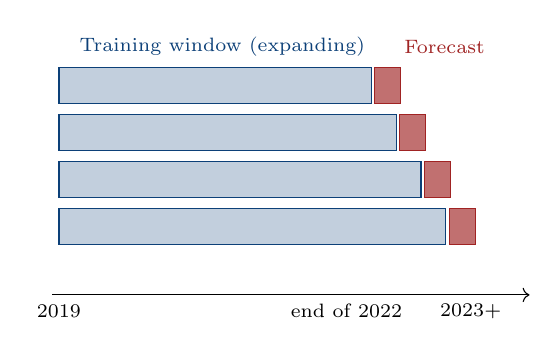
\begin{tikzpicture}[scale=0.83]
        \foreach \i in {1,2,3,4} {
          \pgfmathsetmacro{\tw}{4.4 + \i*0.38}
          \pgfmathsetmacro{\yb}{(5-\i)*0.72}
          \draw[fill=accentblue!25, draw=accentblue]
                (0,\yb) rectangle (\tw, \yb+0.55);
          \draw[fill=accentred!65, draw=accentred]
                (\tw+0.05,\yb) rectangle (\tw+0.45, \yb+0.55);
        }
        \node[font=\scriptsize, accentblue] at (2.5,3.75) {Training window (expanding)};
        \node[font=\scriptsize, accentred]  at (5.9,3.75) {Forecast};
        \node[font=\scriptsize] at (0,  -0.3) {2019};
        \node[font=\scriptsize] at (4.4,-0.3) {end of 2022};
        \node[font=\scriptsize] at (6.3,-0.3) {2023+};
        \draw[->] (-0.1,-0.05) -- (7.2,-0.05);
      \end{tikzpicture}
      \end{center}
      \small FPCA \emph{and} VAR re-estimated at every step.\\
      Only data dated $< d$ used to forecast day $d$.\\[0.3em]
      Mirrors real operational deployment: no information leakage.
    \end{column}
    \begin{column}{0.43\textwidth}
      \textbf{Diebold-Mariano test}\\[0.3em]
      \small Loss differential per observation:
      \[
        d_t = \lvert e_t^{\text{ours}} \rvert - \lvert e_t^{\text{official}} \rvert
      \]
      $H_1{:}\ \mathbb{E}[d_t] < 0$ (our model has lower loss)

      \vspace{0.3em}
      HAC $t$-test on $\bar{d}$
      {\small (Newey-West long-run variance)}\\
      + Harvey--Leybourne--Newbold small-sample correction.

      \vspace{0.3em}
      Run \textbf{pooled} (26,304 obs.)\\
      \phantom{Run }$+$ \textbf{hour-by-hour} (24 tests).

      \vspace{0.3em}
      \small A lower MAE alone is not sufficient evidence.
    \end{column}
  \end{columns}
  \note{The no-leakage principle is paramount. The DM test is a $t$-test on the time-series mean of $d_t$ with a HAC (long-run) variance --- exactly like a Newey-West standard error --- which accounts for serial correlation in forecast errors. The HLN small-sample correction adjusts for finite-sample bias. With 26,304 pooled observations the asymptotic approximation is excellent.}
\end{frame}

% ============================================================
% SLIDE 12: MAIN RESULTS
% ============================================================
\begin{frame}{Preliminary Results: Building the Model Step by Step}
  \begin{center}
  \small
  \begin{tabular}{p{0.40\textwidth}rrrrc}
    \toprule
    Model & MAE & MAPE & vs.\ official & DM stat & \\
    \midrule
    Seasonal na\"{i}ve $Y_{d-7}$  & 1912 & 5.13\% & $-57.6\%$ & $+35.2$ & --- \\
    \textbf{Official (TEİAŞ)}     & \textbf{1214} & \textbf{3.15\%}
                                   & ref. & --- & \\
    \midrule
    FPCA VAR(1,7) only            & 1443 & 3.76\% & $-18.9\%$ & $+22.9$ & \\
    $+$ calendar / ramp           & 1238 & 3.26\% & $-2.1\%$  & $+2.6$  & \\
    \rowcolor{wingreen}
    $+$ holiday / load-shape      & 1001 & 2.63\% & $+17.5\%$ & $-24.9$ & *** \\
    \rowcolor{wingreen}
    $+$ derivative features       & \textbf{980} & \textbf{2.56\%}
                                   & $+19.2\%$ & $-27.4$ & *** \\
    \midrule
    \rowcolor{wingreen}
    $+$ residual correction       & \textbf{653} & \textbf{1.70\%}
                                   & $+46.2\%$ & $-71.2$ & *** \\
    \bottomrule
  \end{tabular}
  \end{center}
  \vspace{0.1em}
  \footnotesize
  *** $p<0.001$ vs.\ official (pooled DM, 26,304 obs.).
  Positive DM stat = worse than official; negative = better.
  MAE in MWh/hour. Evaluation: 2023--2025.
  \note{Walk the table top to bottom. Pure VAR dynamics without features are significantly worse than the official (DM stat +22.9). Calendar/ramp barely helps. The jump comes from holiday + load-shape (MAE 1238 $\to$ 1001, DM stat $-24.9$, $p \approx 10^{-135}$). Derivative features push to 980 (DM stat $-27.4$, $p \approx 10^{-163}$). The residual correction achieves the largest gain (DM stat $-71.2$) but uses a second modelling step on top of the base model.}
\end{frame}

% ============================================================
% SLIDE 13: HOUR-BY-HOUR
% ============================================================
\begin{frame}{Where the Model Wins and Where It Loses}
  \begin{columns}
    \begin{column}{0.60\textwidth}
      \includegraphics[width=\linewidth]{../output/figs/fpca_VAR_1_7_gain_vs_official_by_hour.png}
    \end{column}
    \begin{column}{0.37\textwidth}
      Positive = model beats official (MAE, MWh/hour)

      \vspace{0.6em}
      \textbf{Wins:} hours 0--5 and 10--23\\
      {\small Overnight trough and daytime plateau ---
       stable, weekly-seasonal behavior well captured by VAR lags}

      \vspace{0.5em}
      \textcolor{accentred}{\textbf{Loses:} hours 6--9}\\
      {\small Morning ramp. Demand doubles in 2 hours; ramp timing
        is temperature-driven. At hour 8, our MAPE loss is \textbf{24\%}.}

      \vspace{0.5em}
      \small DM significant at 18 of 24 hours (5\% level).

      \vspace{0.4em}
      \small Persistent, autocorrelated ramp-hour errors motivate the residual correction.
    \end{column}
  \end{columns}
  \note{The ramp-hour loss (6--9) is the key diagnostic. At hour 8, the MAPE loss is 24\% --- the official is 24\% more accurate, almost certainly because it incorporates weather inputs that determine ramp timing. Our model uses only historical load patterns. This gap is not random noise --- it is systematic and autocorrelated, which the residual correction exploits.}
\end{frame}

% ============================================================
% SLIDE 14: RESIDUAL CORRECTION
% ============================================================
\begin{frame}{Residual Correction: Exploiting Persistent Errors}
  \begin{columns}
    \begin{column}{0.56\textwidth}
      \includegraphics[width=\linewidth]{../output/figs/acf_base_vs_correction.png}
    \end{column}
    \begin{column}{0.41\textwidth}
      \textbf{Motivation:} errors are serially correlated\\
      {\small Ljung-Box rejects $H_0{:}\rho_1{=}\ldots{=}\rho_{14}{=}0$
        at all 24 hours. LB stat up to 7,227 at hour 6.}

      \vspace{0.4em}
      \[
        \hat{Y}_d^{\text{res}}(h) = \hat{Y}_d^{\text{base}}(h) + \lambda_d\,\hat{r}_d(h)
      \]
      $\hat{r}_d(h)$: correction curve from recent past residuals\\
      $\lambda_d$: rolling CV on strictly pre-$d$ data --- no leakage

      \vspace{0.5em}
      \textbf{Result:}
      \begin{itemize}
        \item $+46.2\%$ MAE vs.\ official (DM stat $-71.2$)
        \item Wins at \textbf{all 24 hours} including ramp hours
      \end{itemize}

      \vspace{0.2em}
      {\small Gray = base model ACF;\enspace Orange = after correction}
    \end{column}
  \end{columns}
  \note{ACF at hour 6: base model errors ACF $\approx 0.4$ at lag 1, persisting 14+ days. Orange after correction drops sharply toward zero. Holiday periods and seasonal regimes create blocks of consecutive days where the model over- or under-forecasts by similar amounts. The correction curve captures this from strictly past residuals; $\lambda_d$ is tuned by rolling-origin CV. Key result: wins at the ramp hours (6--9) where the base model previously lost.}
\end{frame}

% ============================================================
% SLIDE 15: NONLINEAR EXTENSIONS
% ============================================================
\begin{frame}{Nonlinear Extensions: What the RF Results Suggest}
  \begin{columns}
    \begin{column}{0.55\textwidth}
      \includegraphics[width=\linewidth]{../output/figs/fpca_RF_fixed_mae_by_hour.png}
    \end{column}
    \begin{column}{0.42\textwidth}
      \textbf{Within FPCA structure --- full 2023--2025}\\
      {\scriptsize OLS replaced by RF in score equation; same basis, features, rolling-origin}
      \vspace{0.3em}

      \scriptsize
      \begin{tabular}{lrrc}
        \toprule
        Model    & MAE  & vs.\ off. & DM \\
        \midrule
        Official & 1214 & ref.      & --- \\
        \rowcolor{loserose}
        FPCA-RF  & 1217 & $-0.3\%$  & n.s. \\
        \rowcolor{wingreen}
        FPCA-OLS & \textbf{980}  & $+19.2\%$ & *** \\
        \bottomrule
      \end{tabular}

      \vspace{0.5em}
      \footnotesize
      Within FPCA, OLS outperforms RF --- the linear score
      equation is an effective regulariser.

      \vspace{0.5em}
      \textbf{Bypassing FPCA (Direct RF, 2025 only):}\\
      {\scriptsize Predicts each hour directly from raw features.
        MAE 718 vs.\ official 1052 ($+31.8\%$), FPCA-OLS 910 ($+13.5\%$).\\[0.3em]
        This is a one-year preliminary result --- not directly comparable
        to the 2023--2025 evaluation --- but it suggests that fully
        nonlinear architectures that bypass the functional compression
        may offer further gains. \textbf{Extending this comparison to
        the full three-year window is a key thesis objective.}}
    \end{column}
  \end{columns}
  \note{Two distinct comparisons. (1) Within FPCA: FPCA-RF achieves MAE 1217 (ties official at 1214) while FPCA-OLS achieves 980 --- OLS regularisation wins within the functional structure. (2) Beyond FPCA: Direct RF, which bypasses the FPCA compression entirely, achieves MAE 718 vs.\ official 1052 on the 2025 subsample (+31.8\%) compared to FPCA-OLS's +13.5\% in the same year. This raises an open question: does the FPCA functional structure constrain the model, and would a fully nonlinear approach maintain this advantage over three years? This is the main remaining empirical question.}
\end{frame}

% ============================================================
% SLIDE 16: PROPOSAL SUMMARY
% ============================================================
\begin{frame}{Proposal Summary: Preliminary Findings and Open Questions}
  \begin{columns}
    \begin{column}{0.50\textwidth}
      \textbf{Preliminary findings (proposal phase)}
      \vspace{0.3em}
      \begin{itemize}
        \item FPCA with $K=2$ eigenfunctions represents load curves
              with 97.3\% variance retention; eigenfunctions stable over time
        \item FPCA-VAR with holiday and derivative features achieves
              $+19.2\%$ MAE vs.\ official (DM $p \approx 10^{-163}$,
              2023--2025)
        \item Residual correction brings gains to $+46.2\%$, winning at
              all 24 hours including ramp hours
        \item Within the FPCA structure, OLS outperforms RF, suggesting the
              linear score equation is well-specified for this functional representation
      \end{itemize}
    \end{column}
    \begin{column}{0.48\textwidth}
      \textbf{Open questions for the thesis}
      \vspace{0.3em}
      \begin{itemize}
        \item Does bypassing FPCA entirely (Direct RF, other nonlinear
              architectures) offer sustained gains over the full 2023--2025
              evaluation? The 2025 subsample (+31.8\%) is encouraging but
              based on a single year.
        \item Is the FPCA functional compression a limitation or a feature
              when paired with nonlinear score models?
        \item Can the ramp-hour gap be closed without external weather inputs?
        \item What are the gains from probabilistic forecasting (prediction
              intervals)?
      \end{itemize}
    \end{column}
  \end{columns}
  \note{Frame this slide as what the proposal phase has produced versus what remains genuinely open. The committee should understand that the FPCA-VAR model is a solid baseline with statistically validated gains, but whether fully nonlinear approaches dominate on a fair three-year comparison is an open question that the thesis will address. The 2025 Direct RF result is promising but cannot be taken as definitive.}
\end{frame}

% ============================================================
% SLIDE 17: ROAD MAP
% ============================================================
\begin{frame}{Thesis Road Map}
  \begin{columns}
    \begin{column}{0.48\textwidth}
      \textbf{\textcolor{accentblue}{Proposal-phase analysis (done)}}
      \vspace{0.3em}
      \begin{itemize}
        \item[$\checkmark$] Functional representation (B-splines, FPCA)
        \item[$\checkmark$] Rolling-origin evaluation framework
        \item[$\checkmark$] VAR(1,7) + feature blocks (holiday, derivative)
        \item[$\checkmark$] Residual correction step
        \item[$\checkmark$] DM testing (pooled + hourly)
        \item[$\checkmark$] Eigenfunction stability; $K=4$ check
        \item[$\checkmark$] RF comparison within FPCA (score linearity)
        \item[$\checkmark$] Direct RF --- preliminary, 2025 subsample
      \end{itemize}
    \end{column}
    \begin{column}{0.48\textwidth}
      \textbf{\textcolor{accentred}{Thesis objectives}}
      \vspace{0.3em}
      \begin{itemize}
        \item[$\square$] Systematic literature review
        \item[$\square$] Extend Direct RF to full 2023--2025 evaluation
        \item[$\square$] Investigate nonlinear functional architectures
              (RF, gradient boosting, neural nets on scores)
        \item[$\square$] Ramp-hour diagnostics and write-up
        \item[$\square$] Probabilistic forecasting (prediction intervals)
        \item[$\square$] Thesis write-up
      \end{itemize}
    \end{column}
  \end{columns}
  \note{The completed column is deliberately labelled ``proposal-phase analysis'' rather than ``completed thesis work'' to signal that these are preliminary results. The main empirical questions remaining are: (1) systematic literature review, (2) extending the nonlinear comparison to the full three-year window, and (3) write-up. The Direct RF result on 2025 is in the completed column but explicitly marked as preliminary.}
\end{frame}

% ============================================================
% SLIDE 18: REFERENCES
% ============================================================
\begin{frame}{References}
  \footnotesize
  \begin{thebibliography}{99}

    \bibitem[Kokoszka \& Reimherr(2017)]{kokoszka_2017}
    Kokoszka, P.\ \& Reimherr, M.\ (2017).
    \textit{Introduction to Functional Data Analysis}. CRC Press.

    \bibitem[Diebold \& Mariano(1995)]{dm_1995}
    Diebold, F.X.\ \& Mariano, R.S.\ (1995).
    Comparing predictive accuracy.
    \textit{Journal of Business \& Economic Statistics}, 13(3), 253--263.

    \bibitem[Harvey, Leybourne \& Newbold(1997)]{hln_1997}
    Harvey, D., Leybourne, S.\ \& Newbold, P.\ (1997).
    Testing the equality of prediction mean squared errors.
    \textit{International Journal of Forecasting}, 13(2), 281--291.

    \bibitem[Hyndman \& Ullah(2007)]{hyndman_2007}
    Hyndman, R.J.\ \& Ullah, M.S.\ (2007).
    Robust forecasting of mortality and fertility rates:
    a robust functional data approach.
    \textit{Computational Statistics \& Data Analysis}, 51(10), 4942--4956.

    \bibitem[Xie \& Hong(2016)]{xie_2016}
    Xie, J.\ \& Hong, T.\ (2016).
    GEFCom2014 probabilistic electric load forecasting:
    an integrated solution with forecast combination and residual simulation.
    \textit{International Journal of Forecasting}, 32(3), 1012--1016.

  \end{thebibliography}
\end{frame}

\end{document}
